\reviewer

%% ---------------------- 2.1 ------------------------------

\begin{revcomment}{术语首次出现的中英文全称}
第一次出现 CFLP 应该同时给中文名,然后再在括号中给英文全称和简称。
\end{revcomment}
\begin{revresponse}
感谢您的指正。我们已按照您的建议在全文进行了修改。CFLP 的完整中英文全称“机密联邦学习平台(Confidential Federated Learning Platform, CFLP)”已在其首次出现的位置(引言,第2页,第1段)给出。
\end{revresponse}

%% ---------------------- 2.2 ------------------------------

\begin{revcomment}{1.1.2 节需总结提炼并阐明选择横向的动机}
1.1.2节。这部分对两类联邦学习的介绍需要好好总结和提炼。目前这个表述较为含糊,没有能够清晰的反映出二者的差异。本文为什么要选择横向?动机是什么?有什么意义?这个原因也没有说清楚。
\end{revcomment}
\begin{revresponse}
非常感谢您提出的宝贵意见。根据您的建议,我们对 1.1.2 节进行了认真修改。我们通过增加具象化的例子和对比表格,更清晰地区分了横向与纵向联邦学习;同时,新增段落详细阐述本文选择横向联邦的动机与现实意义。我们相信这些修改使文章的逻辑更加严谨,再次感谢您的指导。
\end{revresponse}

%% ---------------------- 2.3 ------------------------------

\begin{revcomment}{1.1.3 节明确通信机制及其合理性}
1.1.3 节提到选择好的通信机制,那么本文采用什么通信机制?为什么好?没有说清楚。
\end{revcomment}
\begin{revresponse}
非常感谢您提出的宝贵意见。根据您的建议,我们对 1.1.3 节进行了修改,明确本平台采用 gRPC 作为核心通信机制,并从接口定义、传输性能、信道安全及流式数据支持等多个维度,系统性阐述其与联邦学习场景高度契合的技术优势。
\end{revresponse}

%% ---------------------- 2.4 ------------------------------

\begin{revcomment}{1.2.1 节应从共性角度阐述 TEE 基本思想}
1.2.1节。TEE的基本思想显然是泛指TEE技术,那么也包括ARM的TrustZone、CCA,RISC-V的Keystone、AMD的SEV等等,应该从更加抽象的角度阐述TEE防护机制的基本思想。这里用TDX来说明,即便是举例也难以涵盖其他TEE的特点。比如内存加密,这个TrustZone就没有,那么它就不是TEE了吗?因此,既然是泛泛的说,就抓住共性特征,举例也举具有共性特征的例子。至于TDX特有的性质及其应用场景,后面介绍已经有相应的内容了。
\end{revcomment}
\begin{revresponse}
非常感谢您提出的深刻见解。您指出原稿在“TEE 基本思想”的阐述中过于依赖特定技术(如 TDX),未能概括其共性特征。为此,我们重写了 1.2.1 节,聚焦三大核心原则:硬件强制隔离、运行时机密性与完整性保护、以及远程证明;删除过于特定的示例,从通用原理出发并强调保护机制的多样性(如访问控制、内存加密等),以覆盖从 ARM TrustZone 到 Intel TDX 等不同架构。
\end{revresponse}

%% ---------------------- 2.5 ------------------------------

\begin{revcomment}{补充“威胁模型与安全假设”}
论文第2章之前缺乏“威胁模型与假设”这部分的描述,对于敌手能力、系统可能遭受的安全威胁、系统可信边界等划分均不明确,这就为后面所提出的方法和系统到底能提供覆盖何种范围的安全保护带来了不确定性。例如,一般在TEE的应用场景中,所有除TEE之外的区域都是不可信区域,都可能成为攻击者入侵和攻击的对象,那么服务器端、客户端等放在这些区域安全吗?这就会造成整个业务流程的安全防护覆盖不完备,让论文显得存在很多设计纰漏。
\end{revcomment}
\begin{revresponse}
非常感谢您提出的关键意见。我们已在第二章前新增“威胁模型与安全假设”一节:明确定义“诚实但好奇”的中心服务器与不可信网络为主要威胁;划定系统信任边界(客户端与 TEE 可信,服务器宿主与网络不可信);并说明本平台通过构建端到端加密链路实现从可信客户端到可信 TEE 的安全保障,从而在既定威胁模型下实现全流程安全完备性。
\end{revresponse}

%% ---------------------- 2.6 ------------------------------

\begin{revcomment}{第二章相关工作需分类与扩充}
第2章相关工作中,对于如何保证联邦学习计算的隐私性这个话题的论述建议在对相关技术进行总结归纳的基础上,按照小标题进行分类讨论。当前,基于TEE的AI和机器学习相关的论文也不少,这些其实也可以作为相关工作的综述材料。
\end{revcomment}
\begin{revresponse}
感谢您的建议。我们已对第二章进行重组与扩充:独立“隐私攻击”小节,并按差分隐私、密码学与可信执行环境三类展开;在“TEE”小节补充最新研究,涵盖训练完整性、模型知识产权保护与安全并行计算等方向,更清晰引出本文动机。
\end{revresponse}

%% ---------------------- 2.7 ------------------------------

\begin{revcomment}{术语首次出现格式}
第3章第一段第一个词 CFLP 的表述建议先中文再英文:机密联邦学习平台(Confidential Federated Learning Platform, CFLP)。
\end{revcomment}
\begin{revresponse}
感谢您的指正。我们已按建议完成修改。
\end{revresponse}

%% ---------------------- 2.8 ------------------------------

\begin{revcomment}{3.1 节表述需重组并具体化}
    3.1节第一段,这段描写部分用词比较模糊,没有能够说明白到底是什么方法。需要重新进行逻辑组织,并重新对相关涉及内容进行描述。例如:反射形式动态加载,这种描述就显得很虚,看似说了什么,其实什么也没说,读者无法从这些辞藻中获取实际有意义的信息。
\end{revcomment}
\begin{revresponse}
    感谢您的建议。我们已针对3.1节第一段 中“用词比较模糊”的意见进行了修改:我们删除了“反射形式动态加载” 这一模糊表述;并根据项目(联邦模拟平台)的实际机制重写了该段,新描述明确了平台是“根据配置文件”中的运行模式和模型类别,“调用清晰的工厂方法”来实例化相应的“训练器” 与“模型” 组件,从而更准确地阐释了“配置即实验”  的具体工作流程。
\end{revresponse}

%% ---------------------- 2.9 ------------------------------

\begin{revcomment}{3.2 节联邦模拟平台的定位与关系}
3.2节,联邦模拟平台存在意义是什么?和联邦实验平台是什么关系,在实现上相互是什么关系?论文中没有给予足够的体现。从论文的表述来看,联邦模拟平台和实验平台共同构成了CFLP。但是看不到模拟平台和实验平台是如何共同构成CFLP的?他们是如何相互交互调用的?他们是如何部署的?等等,没有足够的体现,这就显得模拟平台在论文中的存在感不强,且没有一个明确可行的实现和部署方案。
\end{revcomment}
\begin{revresponse}
    感谢审稿人的宝贵意见。我们深刻认识到原稿中对联邦模拟平台与联邦实验平台(3.1节与3.2节)关系的阐述不够清晰,导致模拟平台的存在意义未能充分体现。针对此问题,我们已在修改稿第3章的引言部分进行了全面重写和澄清。我们明确了CFLP并非单一的集成系统,而是一个两阶段的研究工作流:联邦模拟平台(3.1节)定位为轻量级的“算法选型”环境,它采用“伪分布式”架构,旨在脱离网络和容器部署的复杂度,高效对比多种算法(如CNN、MLP、KNN等)的基线性能;而联邦实验平台(3.2节)则定位为“部署评估”环境,它承接模拟平台的选型结果(如CNN),在真实的分布式(Docker/gRPC)环境中,专注于量化集成机密计算技术(TEE、HE等)所带来的真实系统开销。因此,两个平台在实现上完全独立,没有直接的交互调用,它们通过研究阶段上的前后承接关系共同构成了CFLP的完整评估体系。
\end{revresponse}

%% ---------------------- 2.10 ------------------------------

\begin{revcomment}{图3与系统可用性、负载均衡与安全机制}
图3,从图中看似乎是多对一的“客户端——服务器”模式,那么并发后如何进行负载均衡?FL Server可能成为系统瓶颈,更容易造成单点失效,其可用性怎么保证?另外,只有核心计算载荷在SGX的Enclave中,那么客户端和服务器端都处于非可信空间吗?他们的运行时安全性由谁保护?另外,系统初始时及运行时客户端和服务器端的身份真实性如何保证?数据传输的机密性如何保证?这些都需要相应的协议和机制来支撑,论文中缺少相关的描述,造成数据和计算安全难以形成全业务周期的闭环,漏洞较多。
\end{revcomment}
\begin{revresponse}
    感谢审稿人的宝贵意见,您指出的可用性、负载均衡和安全闭环问题对于生产级系统至关重要。我们已在修改稿的3.2节中进行了详细澄清,本平台(CFLP)作为一个研究与实验型平台,其设计目标是优先保证实验的可复现性与核心安全机制的验证,而非构建一个生产级的高并发、高可用、高性能系统。针对您提出的具体问题,说明如下:
    
    \begin{itemize}
    \item 关于系统拓扑、瓶颈与可用性:如图3所示,系统确实采用了“多客户端 → 单协调服务端”的星型拓扑。在当前实现中,fl-server是一个单点,这对于保证实验环境的一致性和可复现性是有意的设计。系统并发由gRPC的线程池(max\_workers)处理。我们已在文中申明,生产级的负载均衡与高可用(HA)机制(如多副本协调、选主等)并非本文的研究重点,故未予实现。
    
    \item 关于安全边界与运行时保护: 您是对的,只有核心聚合计算(Aggregation)在TEE(SGX/TDX)的Enclave中执行。我们的威胁模型(1.5节)明确假定客户端环境可信,而服务器端的宿主进程及操作系统均处于非可信空间。因此,系统并不依赖容器隔离来保护服务器运行时,而是通过应用层的端到端加密来保护数据:模型更新在可信客户端加密后,以密文形式“穿透”非可信的服务器宿主进程,最终只在TEE/Enclave内部解密。这确保了宿主进程(即使被攻陷)也无法窃取客户端的明文梯度。
    
    \item 关于身份真实性: 平台提供了分层级的身份验证机制。(1)服务端身份: 系统支持标准TLS加密信道,客户端可通过加载根证书验证服务器身份。(2)TEE(Enclave)身份: 在SGX模式下,服务器会向客户端分发由硬件签名的Quote(包含MRENCLAVE)和Enclave公钥。客户端(在生产环境中)必须通过远程证明验证该Quote的有效性,以确保连接的是未被篡改的聚合程序。(3)客户端身份: 在当前研究环境中,客户端身份仅通过client\_id注册,文中已指出在生产中可通过mTLS等机制增强。
    
    \item 关于数据传输机密性: 我们通过两个层面保障机密性。(1)信道层: gRPC支持TLS传输层加密。(2)应用层: 更重要的是,在所有隐私模式(HE, MPC, TEE/SGX)下,模型参数在离开客户端前就已加密或转换为秘密份额。这意味着,即使TLS信道被攻破(或在开发模式下降级为明文),攻击者截获的也只是无法解密的密文,从而确保了核心数据的端到端机密性。
    \end{itemize}
    
    综上,本平台虽然为实验目的简化了高可用设计,但通过应用层端到端加密和TEE远程证明机制,构建了覆盖数据全生命周期的核心安全闭环,确保了在既定威胁模型下的计算与数据机密性。再次感谢您的宝贵意见。
\end{revresponse}

%% ---------------------- 2.11 ------------------------------

\begin{revcomment}{图4 排版建议}
图4,建议将该大图重新排版,可以分成几个子过程。在文中直接贴Visio的原图从而保证清晰度。
\end{revcomment}
\begin{revresponse}
感谢您的宝贵意见,我们已经按照您的建议重新排版了图4,并将其分成了几个子过程。

\begin{figure}[htbp]
    \centering
    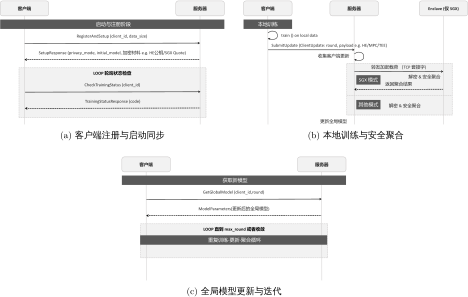
\includegraphics[width=0.9\textwidth]{figures/fig.pdf}
    \caption{修改后的图4 联邦实验平台时序图}
    \label{fig:reorganized_workflow}
\end{figure}

\end{revresponse}

%% ---------------------- 2.12 ------------------------------

\begin{revcomment}{4.3.1 节模拟平台的构成与部署}
4.3.1节,这个模拟平台到底是个什么构成?如何配置和部署的?一直没有详细的描述,这是论文的一个硬伤。
\end{revcomment}
\begin{revresponse}
    感谢您的宝贵意见。您的意见非常中肯,原稿中对联邦模拟平台的描述确实过于抽象,缺少了关键的配置与部署细节,这是一个明显的疏忽。针对此问题,我们对第3.1节 联邦模拟平台(即审稿意见中的4.3.1节)进行了彻底重写。在新版本中,我们详细阐明了模拟平台的核心模块构成(如统一入口、全局配置、训练器、联邦组件等),清晰描述了其在集中式(CL)与联邦(FL)模式下的抽象工作流(特别是联邦训练器如何编排客户端与服务端模块以模拟FedAvg)。并最后分析其作用:为联邦实验平台(3.2节)提供算法选型参考,从而构建一个完整的算法评估与部署体系。
\end{revresponse}

%% ---------------------- 2.13 ------------------------------

\begin{revcomment}{4.4.1 节实验数据分析不足}
4.4.1节,实验数据分析不到位。对实验结果的分析并不是单单看图比较数字的大小,二是要通过这些方法背后的原因、机理来解释为什么会产生这样的结果和差异。
\end{revcomment}
\begin{revresponse}
    感谢审稿专家的宝贵意见。您的批评非常到位,我们确实在原稿中忽视了对实验结果背后机理的深入分析。针对此问题,我们对第4.4.1节的分析部分进行了补充。在新版本中,我们不再仅仅比较数字,而是着重从模型架构(如CNN的空间捕捉能力为何优于MLP和LR)、算法机理(如FedAvg的加权平均机制为何能天然对抗“数量偏斜”)以及数据分布特性(等角度,详细解释了实验结果差异产生的原因。
\end{revresponse}

%% ---------------------- 2.14 ------------------------------

\begin{revcomment}{图6 可读性}
图6,图中坐标轴文字、柱状图上的文字太小,可读性差。
\end{revcomment}
\begin{revresponse}
感谢您的宝贵意见。我们已经使用 Python 的 Matplotlib 库重新绘制了图 6,以提高其可读性。新图表的字体大小和清晰度都得到了优化。
\begin{figure}[htbp]
    \centering
    \includegraphics[width=0.9\textwidth]{figures/figure_6_remake.pdf}
    \caption{修改后的图6 联邦模拟平台实验结果柱状图}
    \label{fig:reorganized_workflow}
\end{figure}
\end{revresponse}

%% ---------------------- 2.15 ------------------------------

\begin{revcomment}{4.4.2 节类似问题}
4.4.2节,与4.4.1节类似问题,和上面一样,对实验结果的分析不足。
\end{revcomment}
\begin{revresponse}
    感谢审稿专家的宝贵意见。我们完全同意您提出的“原稿对实验结果的分析确实流于表面,未能揭示数据差异背后的机理”。针对此问题,我们对第4.4.2节进行了彻底重写。在新版本中,我们重新分析了五种策略在计算效率和通信开销上产生巨大差异的根本原因:例如,HE的耗时瓶颈在于客户端的Paillier加密(模幂运算),其通信膨胀(x128)源于4字节明文到512字节密文的固定扩张;而TEE方案(TDX/SGX)的通信开销与基线持平,则得益于混合加密机制(AES密文等长)。我们相信,这些基于技术机理的分析能更充分地支撑本文的结论。
\end{revresponse}

%% ---------------------- 2.16 ------------------------------

\begin{revcomment}{安全性分析的补充}
第4章除了性能分析之外,还需要进行安全性分析,即本文机制如何就能保障计算的全业务周期安全?怎么实现对计算、传输、存储的机密性、完整性保护?怎么实现对参与方身份真实性的验证?
\end{revcomment}
\begin{revresponse}
    感谢审稿专家的宝贵意见。您指出的原稿缺少安全性分析确实是本文的一大疏漏。针对此问题,我们已在第四章中增补了“4.5 安全性分析”一节。该章节详细论述了本平台如何基于第1.3节的威胁模型与安全假设,在计算、传输和存储这三个全业务周期中提供安全保障。具体而言,我们分析了HE、MPC和TEE三种策略如何分别实现安全的“聚合计算”;阐释了“信道层TLS”与“应用层端到端加密”的双重机制如何保障“传输安全”;说明了服务器临时“存储”的数据为何始终保持加密状态;最后,我们还详细介绍了平台如何通过TLS证书和TEE远程证明(Remote Attestation)机制来保障“参与方身份的真实性”。
\end{revresponse}

\begin{concludingresponse}[]
感谢审稿专家的系统性建议,我们已根据所有意见完成了论文的结构重构与内容增补。
\end{concludingresponse}
